\problemname{\problemyamlname}

\illustration{0.3}{luggage}{Suitcase size check. \href{https://commons.wikimedia.org/wiki/File:Wizz_Air_and_Ryanair_baggage_sizer.jpg}{Photo by Kenzel2}\vspace{-0.5cm}}%
You want to travel to the Olympic Games this year and already decided to take the Eurostar to Paris to be more environmentally friendly.
Your next decision is to pick a suitcase for your journey.
Upon reading the terms and conditions, you noticed that there is no clear size limit for the suitcase.
Instead, they provide various two-dimensional constraints, and your suitcase is compliant if it fits in a box where each side matches one of the aforementioned constraints.

\begin{figure}[!h]
	\centering
	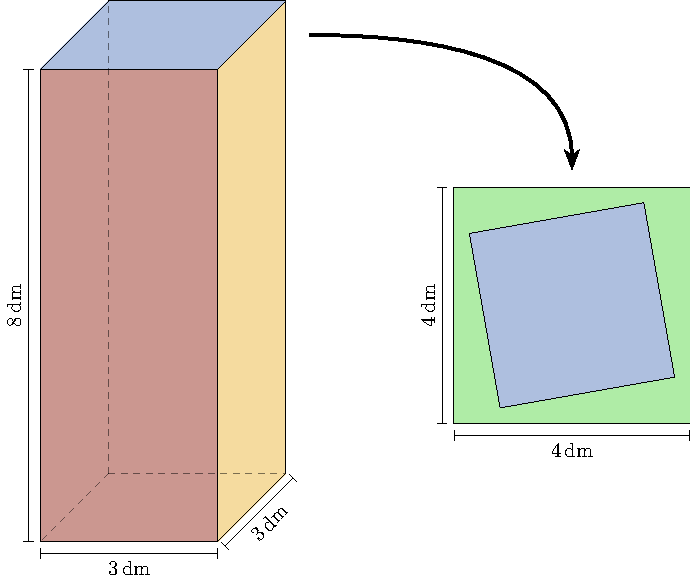
\includegraphics[width=0.4\textwidth]{sample2}
	\caption{Illustration of Sample 2.
		A suitcase with dimensions $3 \textrm{dm}\times8 \textrm{dm}\times3 \textrm{dm}$ fits in a box where each side has either dimension $3\textrm{dm}\times8\textrm{dm}$ or $4\textrm{dm}\times4\textrm{dm}$, i.e.\ complies either with constraint $3$ or $1$ of the input.}
\end{figure}

Since you need to buy a new suitcase anyway, you wonder how much volume could a suitcase have and still be compliant?

\begin{Input}
	The input consists of:
	\begin{itemize}
		\item One line with an integer $n$ ($1\leq n\leq 2\cdot10^5$),
		the number of constraints.
		\item $n$ lines, each containing two integers $a$ and $b$ ($1\leq a,b\leq10^6$), the dimensions of the constraint in $\textrm{dm}$.
	\end{itemize}
\end{Input}
\begin{Output}
	Output a single integer, the maximum volume of a suitcase that you can carry with you in $\textrm{dm}^3$.
\end{Output}
